\documentclass{article}
\title{Projet de fin d'études}
\author{Ian Gruson}
\date{Janvier 2021}

\usepackage{float}
\usepackage{graphicx}
\usepackage{hyperref}
\usepackage{color}
\usepackage{listings}
\usepackage{pdfpages}

\begin{document}
\maketitle
\begin{center}
\large\textbf{Tuteur de stage : Patrick Bard}\\
\vspace*{\stretch{1.0}}
\large\textbf{Enseignant référant : Jérôme Rossignol}

\end{center}
\vspace*{\stretch{1.0}}
\begin{center}
\large\textbf{ESIREM}\\

\includegraphics[scale=0.7]{images/logoEsirem}\\
\vspace*{\stretch{1.0}}
\large\textbf{Promotion Pascal}
\vspace*{\stretch{1.0}}\\
\large\textbf{LEAD}\\
% \includegraphics[scale=0.7]{images/logoi3mainz}\\
\large\textbf{Intitulé de la mission : Développement d'un générateur de figures de Navon}
\end{center}
\vspace*{\stretch{2.0}}
\newpage
\renewcommand{\contentsname}{Sommaire}
\tableofcontents
\newpage
\renewcommand{\listfigurename}{Liste des figures}
\listoffigures
\newpage
\section{Remerciements}
J'aimerai remercier les professeurs de l'ESIREM pour leurs enseignements au travers de ces trois années d'école. En particulier je voudrai remercier M. Sergey Kirgizov pour sa pédagogie, sa bienveillance et son soucis du bien être de ses étudiants. Suivre ses cours fut toujours un plaisir.

\newpage
\section{Présentation de l'entreprise}
	Le Laboratoire d'étude de l'apprentissage et du développement (LEAD) est un laboratoire de recherche axé sur la psychologie cognitive basé sur Dijon. Le Laboratoire étudie notamment les modifications de processus de traitement de l'information consécutives aux apprentissages et au développement. Il est rattaché a l'Institut des Sciences Biologiques (INSB) du Centre National de Recherche (CNRS). Il est constitué de 13 enseignants-chercheurs (7 PU, 6 MCU), 2 chercheurs CNRS (1 DR, 1 CR), 2 ITA et 2 BIATSS, auxquels s’ajoutent 3 chercheurs visiteurs (1 DR, 1 PU, 1 MCU), 8 chercheurs associés (dont 1 DR, 1 PU, 2 MCU), 4 ingénieurs contractuels autofinancés, et 8 doctorants. 

	\section{Mission du stage}
	Un des test sur l'apprentissage implicite et explicite très connu dans le monde de la psycologie cognitive est le test des figures de Navon. Une figure de Navon s'agit classiquement d'une forme de lettre de l'alphabet formé d'une autre lettre de l'alphabet plus petite. Par exemple, il faut imaginer une grande lettre A (que l'on appelle comunément lettre globale) dessiné à partir de petite lettre b (qui est la lettre locale). Le test s'effectue en montrant à un candidat une série de figures de Navon auquel il doit répondre rapidement par la lettre locale qu'il voit. Le test n'est évidemment pas simple car par réflexe le candidat aura plutôt tendance à se focaliser sur la lettre globale.
	Pour effectuer un test, il convient d'avoir un nombre de figures important et varier afin d'avoir des résultats plus fiable. Or à ce jour il n'existe pas d'outils permettant de générer de façon simple et rapide ces figures, et les chercheurs du LEAD sont contraints de les créer à la main sur un tableur. 
	La mission de ce stage était donc de produire un logiciel simple d'utilisation qui permettrait aux chercheurs de générer une multitudes de figures rapidement et de façon configurable. 

	\section{Précédents travaux}
	La mission a été confié à un autre étudiant en DUT l'année passée, et l'approche qui avait été privilégié était de configurer les figures à partir de fichiers json contenant des points en coordonnées cartésiennes. Ces points permettaient ensuite de tracer les lettres locales suivant des droites. Pour un A il faut 5 points représentant 5 sommets pour tracer trois droites.


	\section{Approche actuelle}
	\subsection{génération des figures}
	L'approche qui fut développé dans ce travaux, était d'utiliser des listes de 0 et de 1 (bitmap) pour former les lettres globales (Mettre exemple, ici). la taille de la liste correspond à la resolution de la figure de Navon. Pour chaque 1 dans la liste le générateur imprime un caractère ou une lettre, et pour chaque zéro il n'imprime rien. La taille des listes étant bien évidemment modifiable, il est possible des créer des formes plus ou moins complexes. 


	\begin{figure}[!h]
		\centering
		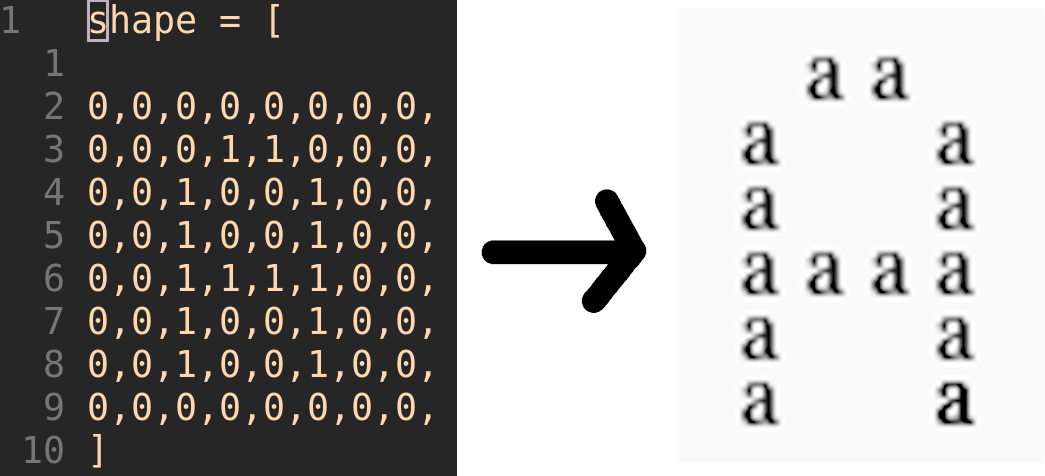
\includegraphics[scale=0.9]{./images/txt_to_image.png}
		\caption{exemple d'un bit array d'une figure représentant un A majuscule}
	\end{figure}

	\subsection{génération des bits array}

En partant de cette base pour générer des figures, il faut encore pouvoir générer les bits array rapidement et sans difficultés afin de simplifier la tâche des psychologues. Alors la création d'une application graphique pour ordinateur était nécessaire. L'application a été développé en C++ avec l'API Qt. Cette combinaison de technologies permet sa grande portabilité sur différents systèmes d'exploitations (Windows, Linux et MacOS) grâce au C++, et une grande modularité dans la création de widget graphiques avec Qt. 

Le principe de l'application est d'afficher un canevas sur lequel l'utilisateur peut venir dessiner ses figures de Navon, et génerer des fichiers textes contenant les bit arrays. Il pourra par la suite générer les images à partir de ces fichiers à l'aide d'un bouton sur l'interface. 
	L'idée du canevas pour dessiner les figures s'inspire des applications comme Piskel (fig:\ref{fig:Piskel}) qui permettent de créer des sprites de jeux vidéos en pixel art (8bits, 16 bits, 32 bits, etc...). Cette manière de dessiner à pour avantage son extrême simplicité d'utilisation et de prise en main, et s'accorde parfaitement aux bits arrays qui sont générés.

	\begin{figure}[!h]
		\centering
		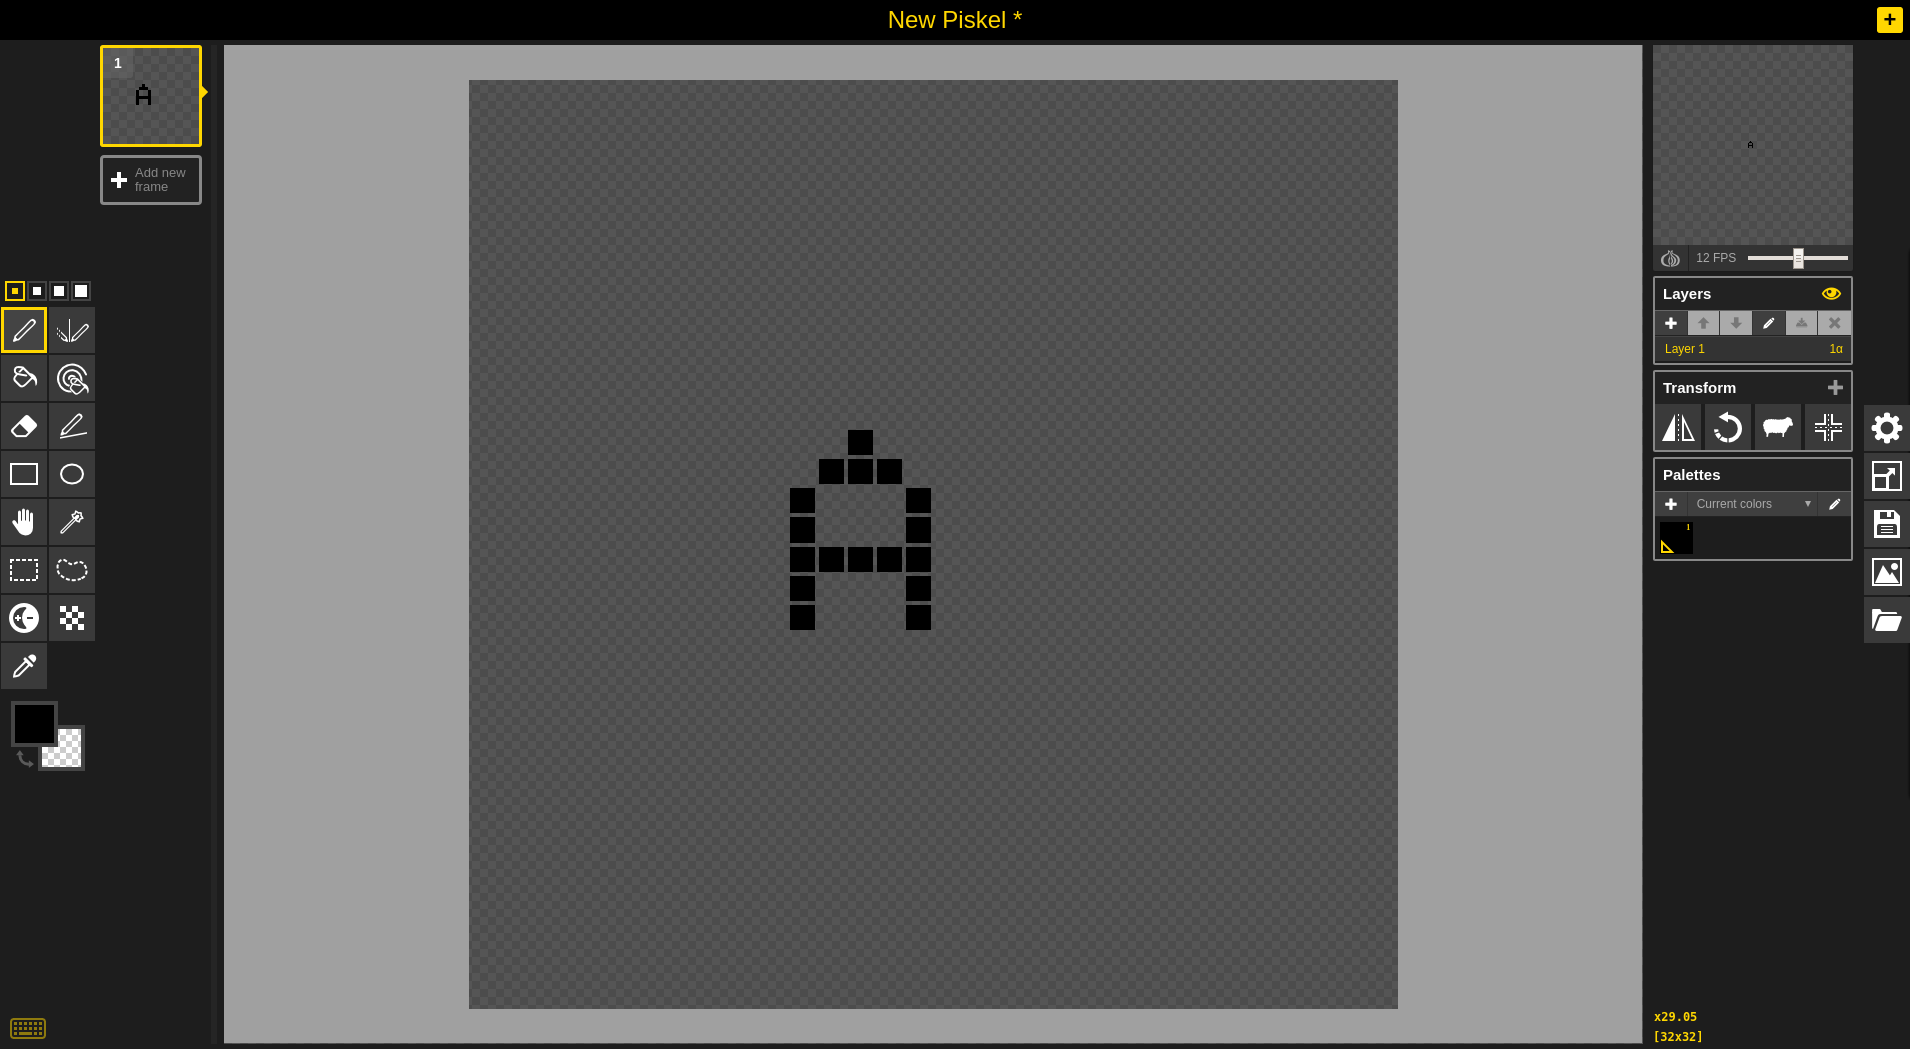
\includegraphics[scale=0.2]{./images/piskel.png}
		\caption{interface de l'application Piskel}
		\label{fig:Piskel}
	\end{figure}

	Comme pour Piskel, l'application affiche un canevas sur lequel l'utilisateur peut cliquer et afficher des carrés noirs. Pour chaque carrés noirs affichés sur le canevas, un bit passera un 1 dans le bit array au même index (fig : \ref{fig:canevas_array}). 

	\begin{figure}[!h]
		\centering
		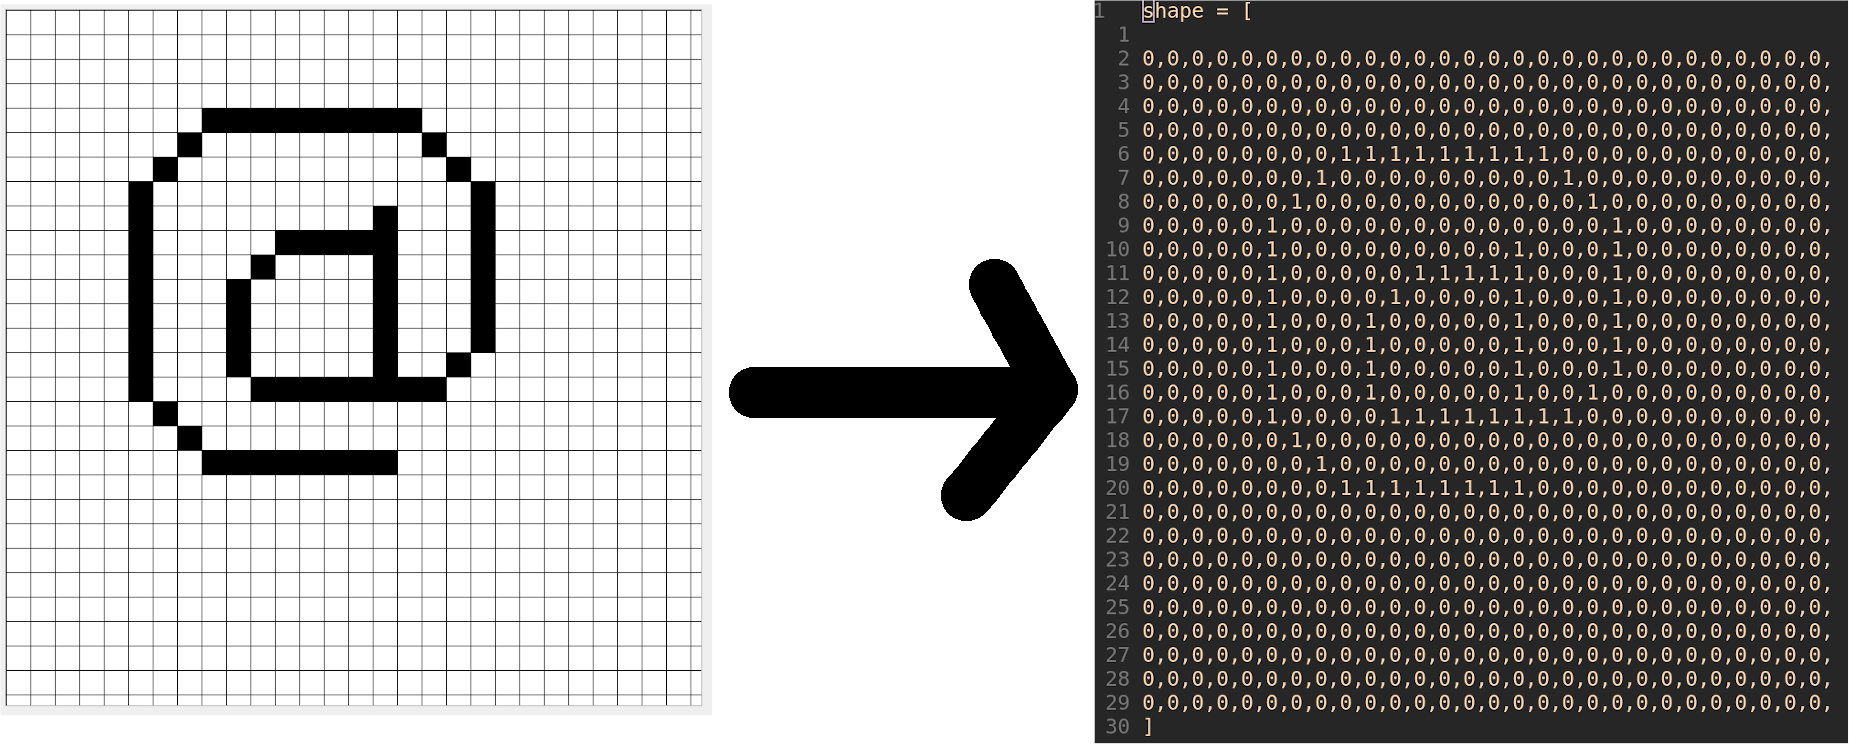
\includegraphics[scale=0.8]{./images/grid-txt.png}
		\caption{exemple de la génération du bitArray depuis la grille}
		\label{fig:canevas_array}
	\end{figure}

	\newpage
	\section{Diagrammes UML}
	\subsection{Diagramme cas d'utilisation}

	\begin{figure}[!h]
	L'application devra à minima suivre ce diagramme d'utilisation. L'utilisateur peut dessiner la figure sur l'interface ainsi que modifier les paramètre de génération de l'image. La génération de l'image qui est gérer par l'application dépend de la génération des fichiers textes. Tandis que la génération des fichiers de textes dépends des dessins de l'utilisateur. D'autres fonctionnalités peuvent s'ajouter par la suite afin d'aller plus loin dans le confort d'utilisation et la flexibilité d'édition. 
	
		\centering
		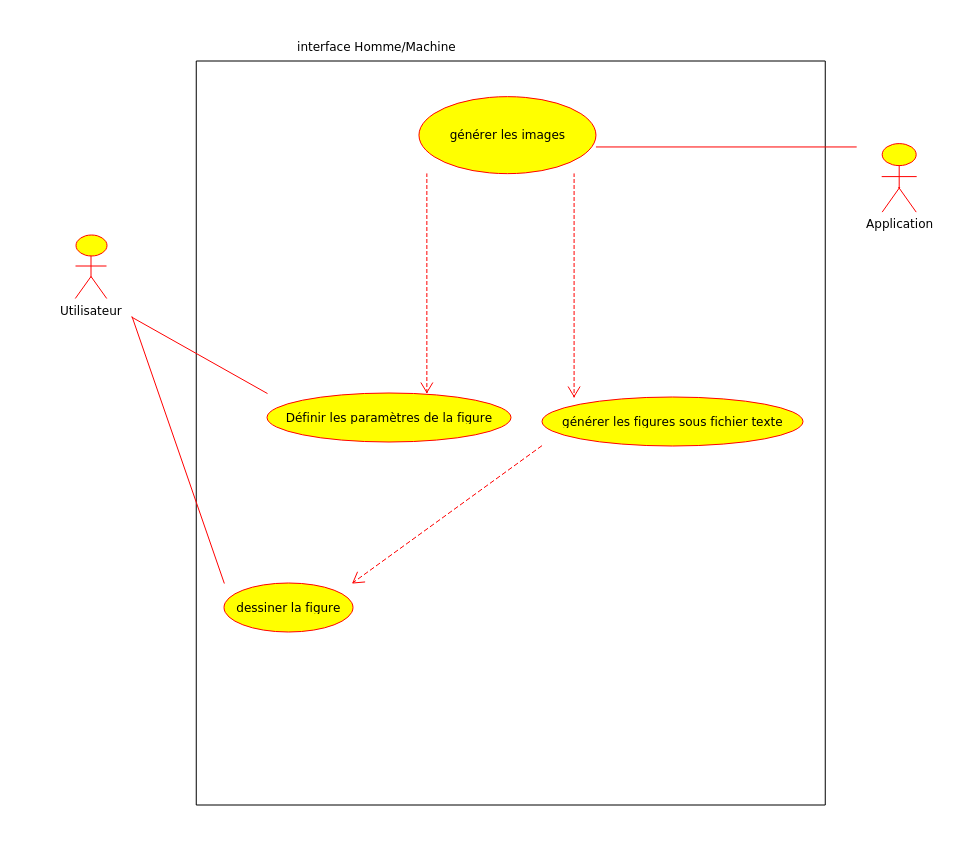
\includegraphics[scale=0.35]{./images/diagramme_cas_utilisation.png}
		\caption{diagramme de cas d'utilisation du générateur.}
		\label{fig:utilisation}
	\end{figure}

	\subsection{Diagramme de classes}
	% Diagramme UML de la figure de Navon
	Le diagramme de classes du générateur est le suivant (fig : \ref{classe_figure}). Le constructeur de la classe navonFigure prends le caractère local, la taille de police, et l'espacement pour gérer la densité des caractères. La classe gridCanvas, qui affiche le canevas sur lequel l'utilisateur peut dessiner ses figures, comporte trois attributs : canvasWidth (la taille du canvas en pixel), sizeOfCell (la taille d'une case/cellule), et numberOfCells (le nombre de cases/cellules, soit la résolution de la grille).

	\begin{figure}[!h]
		\centering
		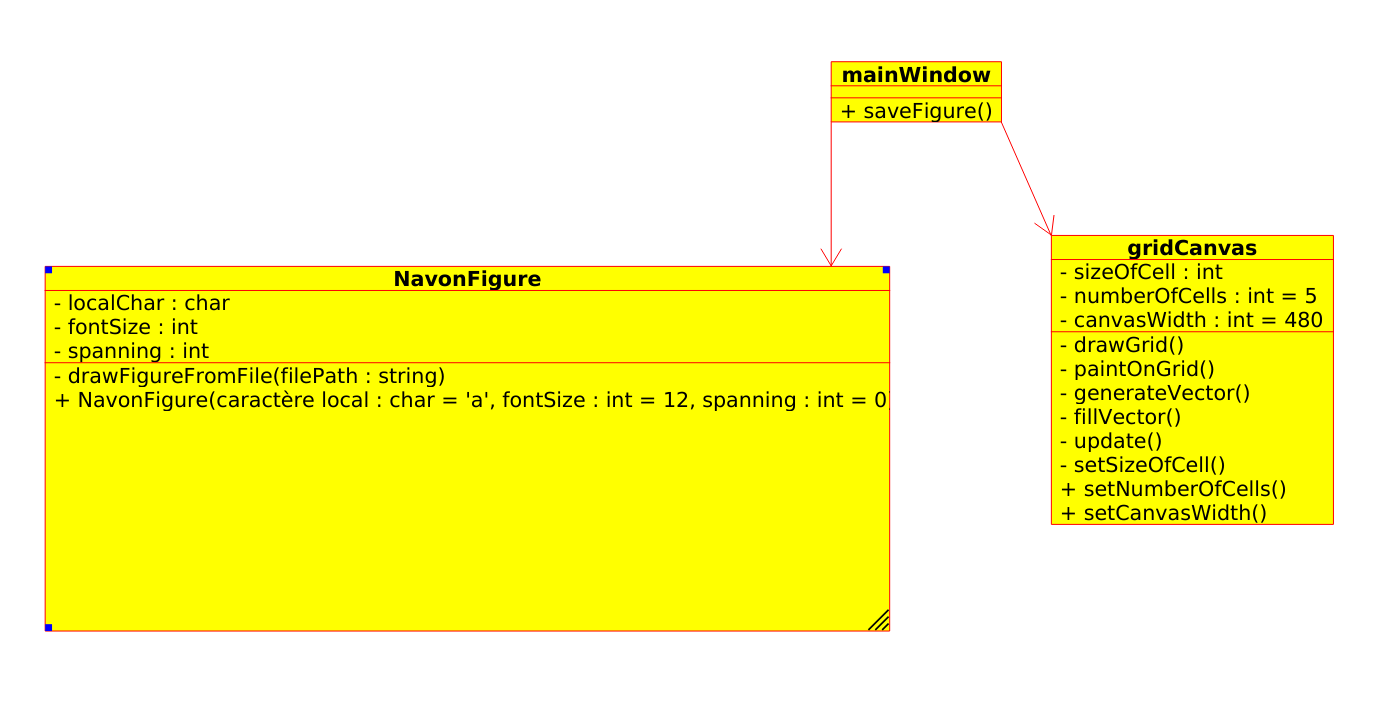
\includegraphics[scale=0.25]{./images/diagramme_classe.png}
		\caption{diagrame de classes du générateur}
		\label{fig:classe_figure}
	\end{figure}

	\section{Présentation de l'application}
	La figure\ref{fig:interface} présentée ci-dessous correspond à l'interface de l'application telle qu'elle est à ce jour. L'utilsateur est directement présenté face à la grille de dessin ainsi que quelques boutons et slider. Toute la partie gauche de l'interface est consacrée à la grille et à la génération des fichiers textes. Il y a deux sliders : le premier permet de d'agrandir ou de rétrécir la zone de dessin, tandis que le deuxième modifie le nombre de cases/cellules de la grille. Enfin il y a un bouton "create .txt file" qui permet à l'utilisateur de choisir le chemin du fichier texte et de le générer. La partie droite de l'application se concentre sur la génération des images à partir des fichiers textes. L'utilisateur choisit d'abord le fichier texte contenant la (ou les) figure de Navon, puis il choisit les paramètre (taille de police, espacement entre les lettres, et caractère local). Enfin il peut générer son image en cliquant sur le bouton "generate image" qui ouvrira un explorateur de fichier, où il devra spécifier le chemin de son image.

	\begin{figure}[!h]
		\centering
		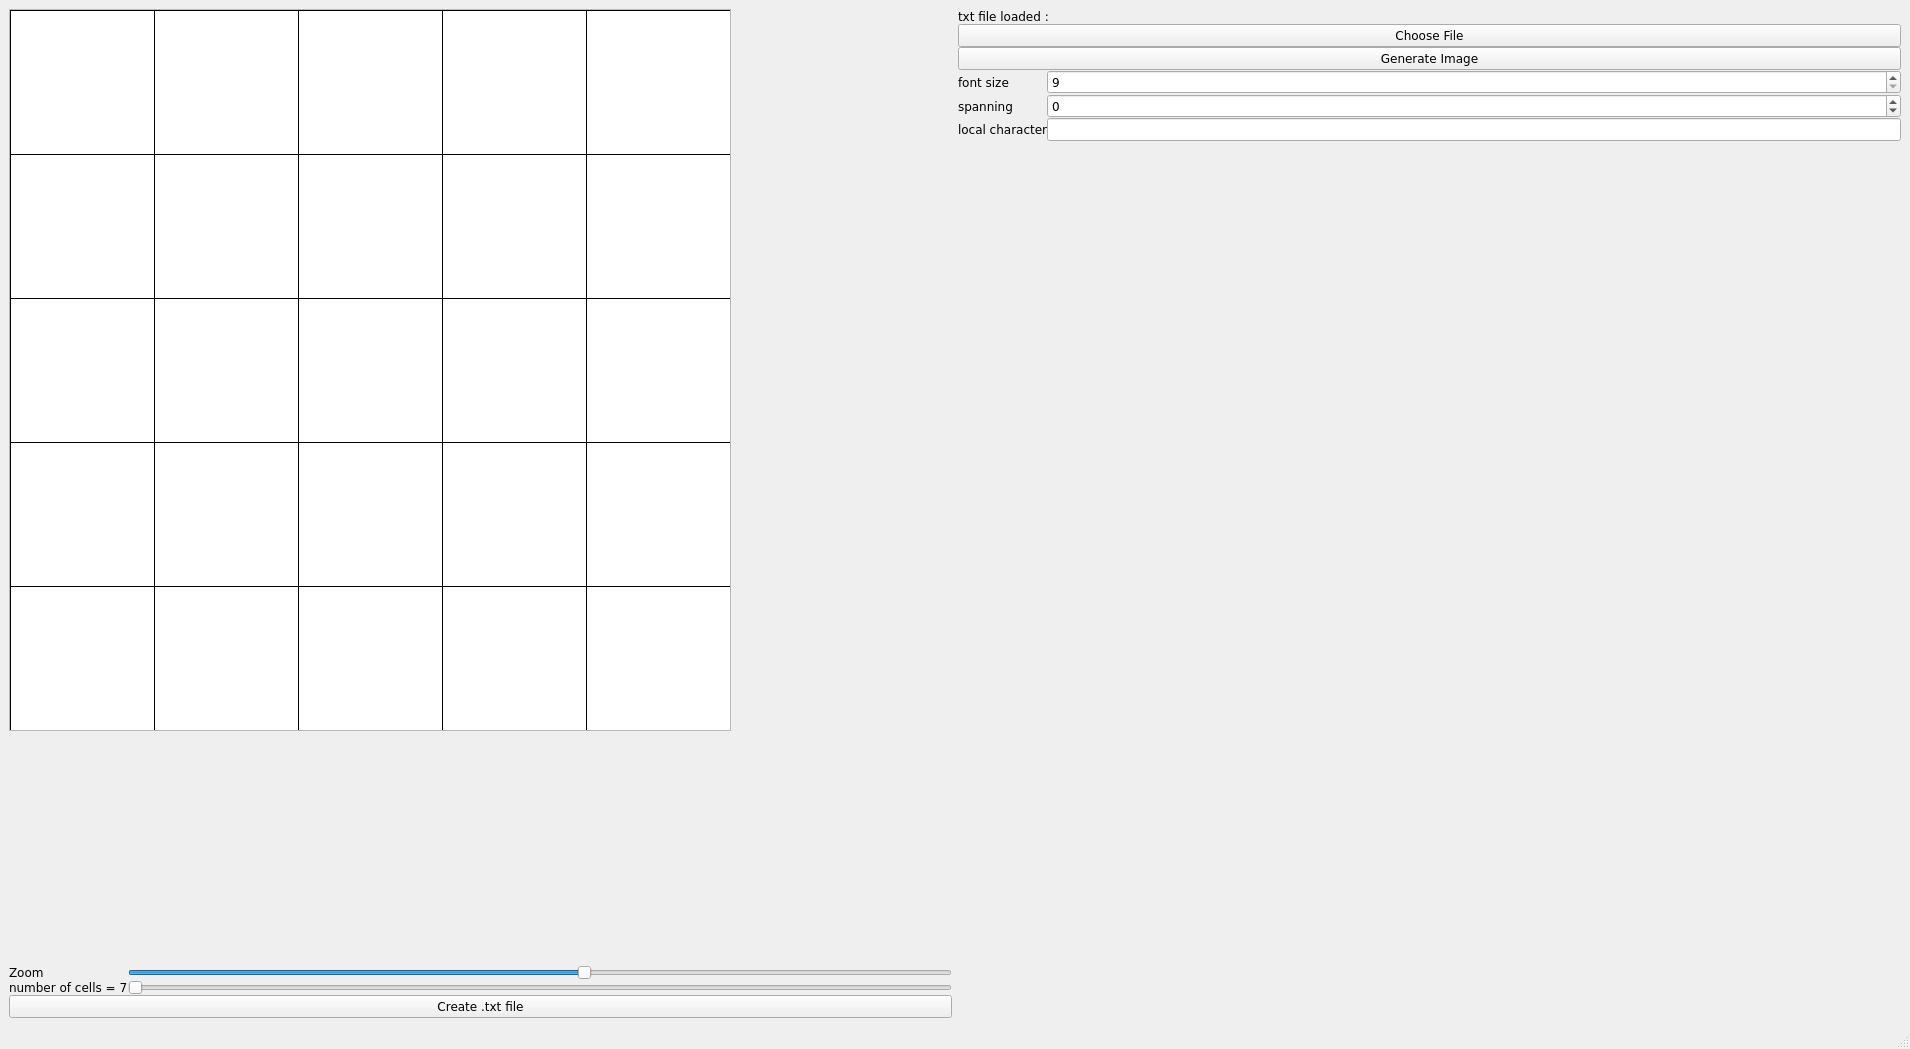
\includegraphics[scale=0.2]{./images/interface.png}
		\caption{interface de l'application}
		\label{fig:interface}
	\end{figure}

	\section{Application}
	En plus d'aider les chercheurs du LEAD dans leurs travail, cette application pourra profiter à d'autres pyschologues à travers le monde. En effet plusieurs options sont envisageable : L'application pourra être publiée en open-source sur des platerformes telles que github ou gitlab, ou être vendue sous la forme d'éxecutable. 

	\section{Conclusion}
	Pour conclure, l'application est fonctionnelle, et dessiner les figures sur la grille est simple et rapide même avec énormément de cases. Cette approche possède une limite néamoins, il n'est pas possible de dessiner des courbes ou des cercles. La meilleur façon d'approcher des courbes est d'augmenter le nombre de cases et les dessiner à la main. Une résolution suffisante de cases peut aisément donner l'impression de courbure. Bien que l'application soit utilisable, elle mériterait néamoins d'être améliorée et peaufinée. En effet, quelques fonctionnalités peuvent s'ajouter pour augmenter son intérêt. La plus évidente et la possibilité de recharger le dessin sur la grille à partir d'un fichier texte existant pour modifier une figure. À ce jour, pour effectuer des petites modifications sur une figure il faut le modifier directement dans le fichier texte. Une autre fonctionnalité qui n'a pas eu le temps d'être implémentée est la possibilité d'effacé un carré noir sur le canevas à l'aide d'un clic droit de la souris par exemple. Pour l'instant les sliders réinitialise le canevas.
	
	Sur le plan personnel, créer cette application de toute pièce fut amusant, et instructif. J'ai pu mieux prendre en main Qt que par le passé et j'ai réussi à franchir le pic de difficulté initial. En effet Qt est un framework extrêment dense et puissant et comprendre le fonctionnement des différents objets qu'il propose réprésente ce pic de difficulté initial. J'ai néamoins trouvé ce projet amusant car j'ai du faire preuve de créativité pour arriver à ce résultat. De plus faire des programmes informatiques reste toujours un plaisir pour moi. 

	\newpage
	\section{Bibliographie}
	Des tentatives de recherches ont été faites, et bien que les figures de Navon ont vu bien des papiers scientifiques écrits à leurs sujet, rien en lien avec de la génération ou l'informatique n'a été trouvé. Aucun papier scientifique n'a été utilisé pour produire l'application et rédiger ce rapport.

	Seul mention à Piskel qui est open-source, qui m'est utile lorsque je développe des jeux vidéos en pixel art et qui m'a servit d'inspiration pour le canevas de l'application.
	Piskel https://www.piskelapp.com/






\end{document}
